As mentioned in previous sections, our ion trap continually holds the ions initially loaded, as well as the subsequent charged reaction products (within the trappable mass range). This feature (bug) is of particular importance for us, as we cannot directly read off the ratio of the isomers and will need to contend with the possibility that the two isomers will continually react with \ce{H2O} at different rates:

\begin{align}
	\ce{HCO+ + H2O & -> H3O+ + CO} \label{r: HCO+H2O->H3O} \\
	\ce{HOC+ + H2O & -> H3O+ + CO} \label{r: HOC+H2O->H3O}
\end{align}

Theoretically, the differing dipole moments of the isomers would produce different dipole-dipole interactions with \ce{H2O}. Literature shows that averaged dipole moments for \ce{HCO+} and \ce{HOC+} are 4.6 D and 2.4 D, respectively.\cite{Rogers1982} But these contribute the a dipole dipole rate constant contribution, which is very short ranged ($1/r^6$) and do not contribute much to the overall rate constant.

We cannot deterministically measure the rate of reaction \ref{r: HOC+H2O->H3O} because there is not a way to produce only \ce{HOC+}, but we may produce only \ce{HCO+}. Considering reactions \ref{r: X+HOC->HCO} and \ref{r: X+HOC->XH}, if we let \ce{X = CO}, we find that both reactions can only yield \ce{HCO+}, allowing us to deterministically produce one of the isomers:

\begin{equation}
\ce{HOC+ + CO -> HCO+ + CO} \label{r: HOC+CO->HCO}
\end{equation}

By producing only \ce{HCO+}, we directly observe reaction \ref{r: HCO+H2O->H3O} with a multi-step reaction procedure. With loaded \ce{Be+} and \ce{C+}, the trap is exposed to \ce{H2O} from the CBGB, to produce a combination of the isomers \ce{[HCO]+}, all the while, \ce{CO} is introduced via the leak valve in the differential cross region to a pressure of $\approx 4 \times 10^{-9}$ Torr as measured in the trap chamber. The constant introduction of \ce{CO} ensures full conversion of \ce{HOC+ -> HCO+} at a rate $\approx \times 10$ faster than that of reactions \ref{r: C+H2O->HCO} and \ref{r: C+H2O->HOC} ensuring we are seeing the time evolution of reaction \ref{r: HCO+H2O->H3O} as seen in Figure \ref{fig: [HCO]+H2O rate}b). A similar procedure of continuously exposing the trap to the CBGB without \ce{CO} yields a combination of the rates of reactions \ref{r: HCO+H2O->H3O} and \ref{r: HOC+H2O->H3O} seen in Figure \ref{fig: [HCO]+H2O rate}a).

The rates of reactions \ref{r: C+H2O->HCO}, \ref{r: HCO+H2O->H3O}, and a combination of reactions \ref{r: HCO+H2O->H3O}+\ref{r: HOC+H2O->H3O} are found with least-squares fitting of the solutions to differential equations found in section \ref{sec: C+H2O eqs}. Beam densities are determined for each run individually by considering the \ce{Be+ + H2O} reaction complex as outlined in Section \ref{sec: trap beam density}.

\begin{figure}[H]
	\centering
	\makebox[\textwidth][c]{
	\begin{tabular}{cc}
		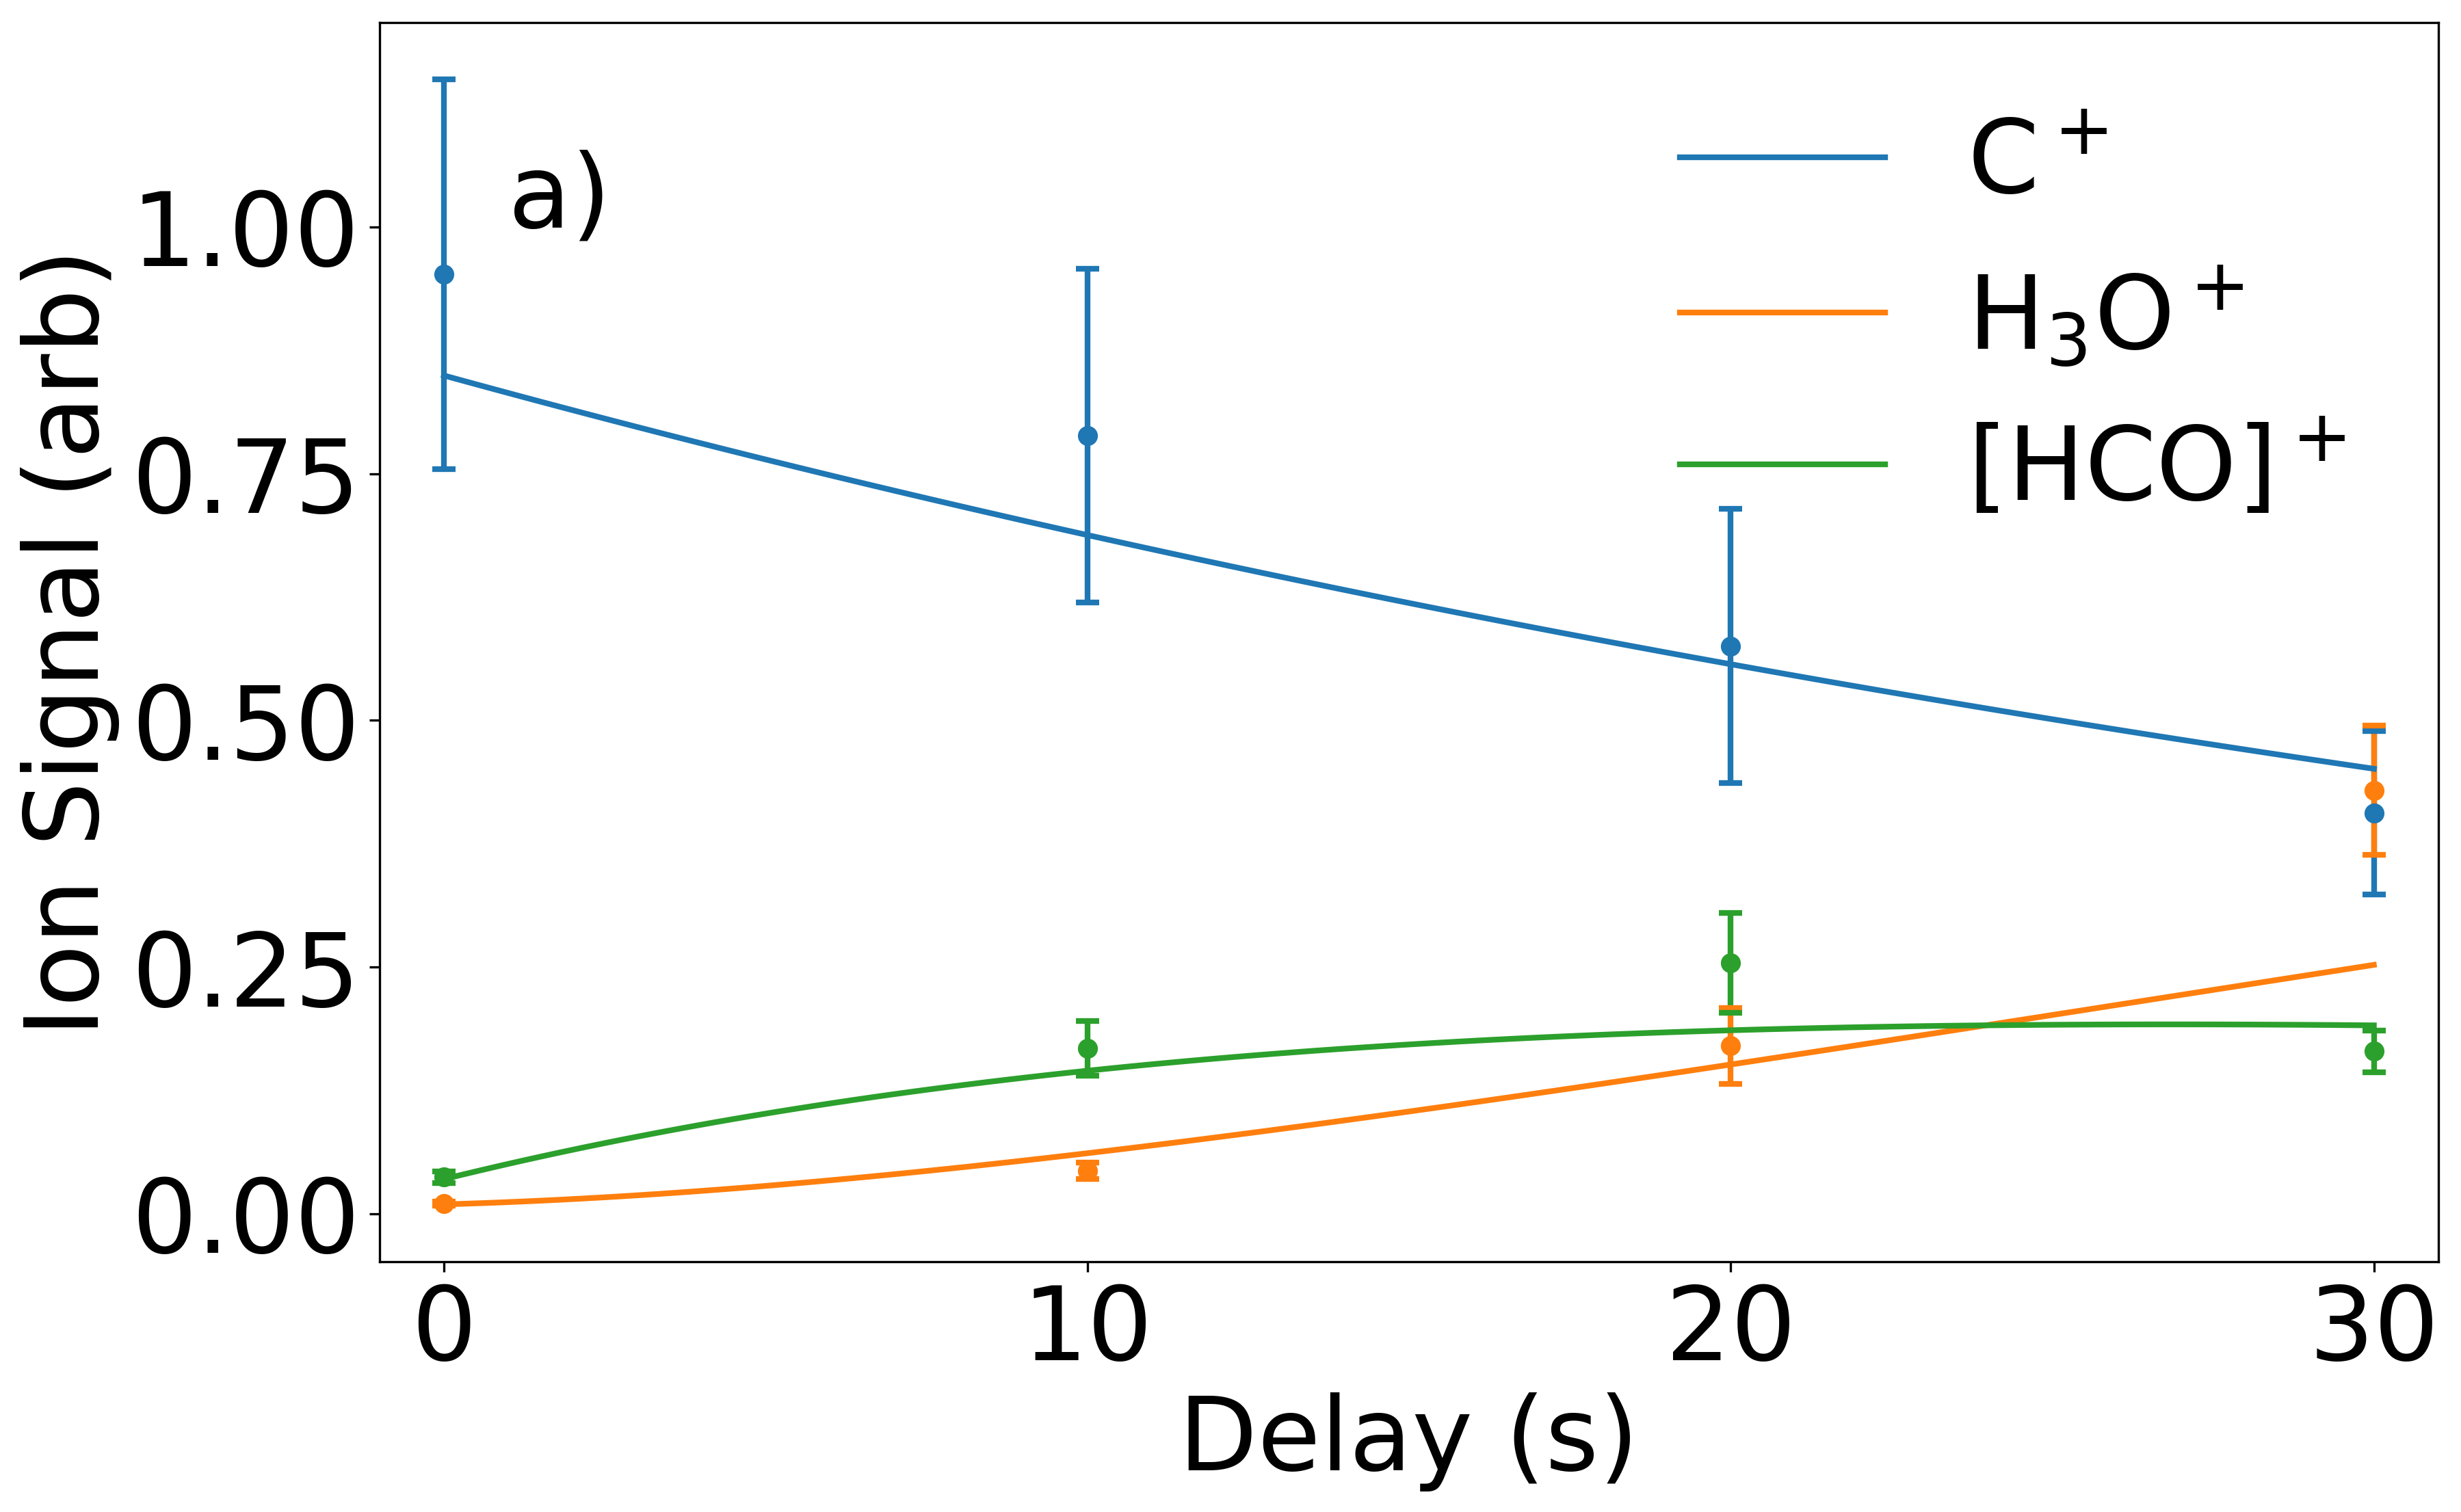
\includegraphics[width=0.5\textwidth]{images/C_H2O_beam_traces_small.png} &
		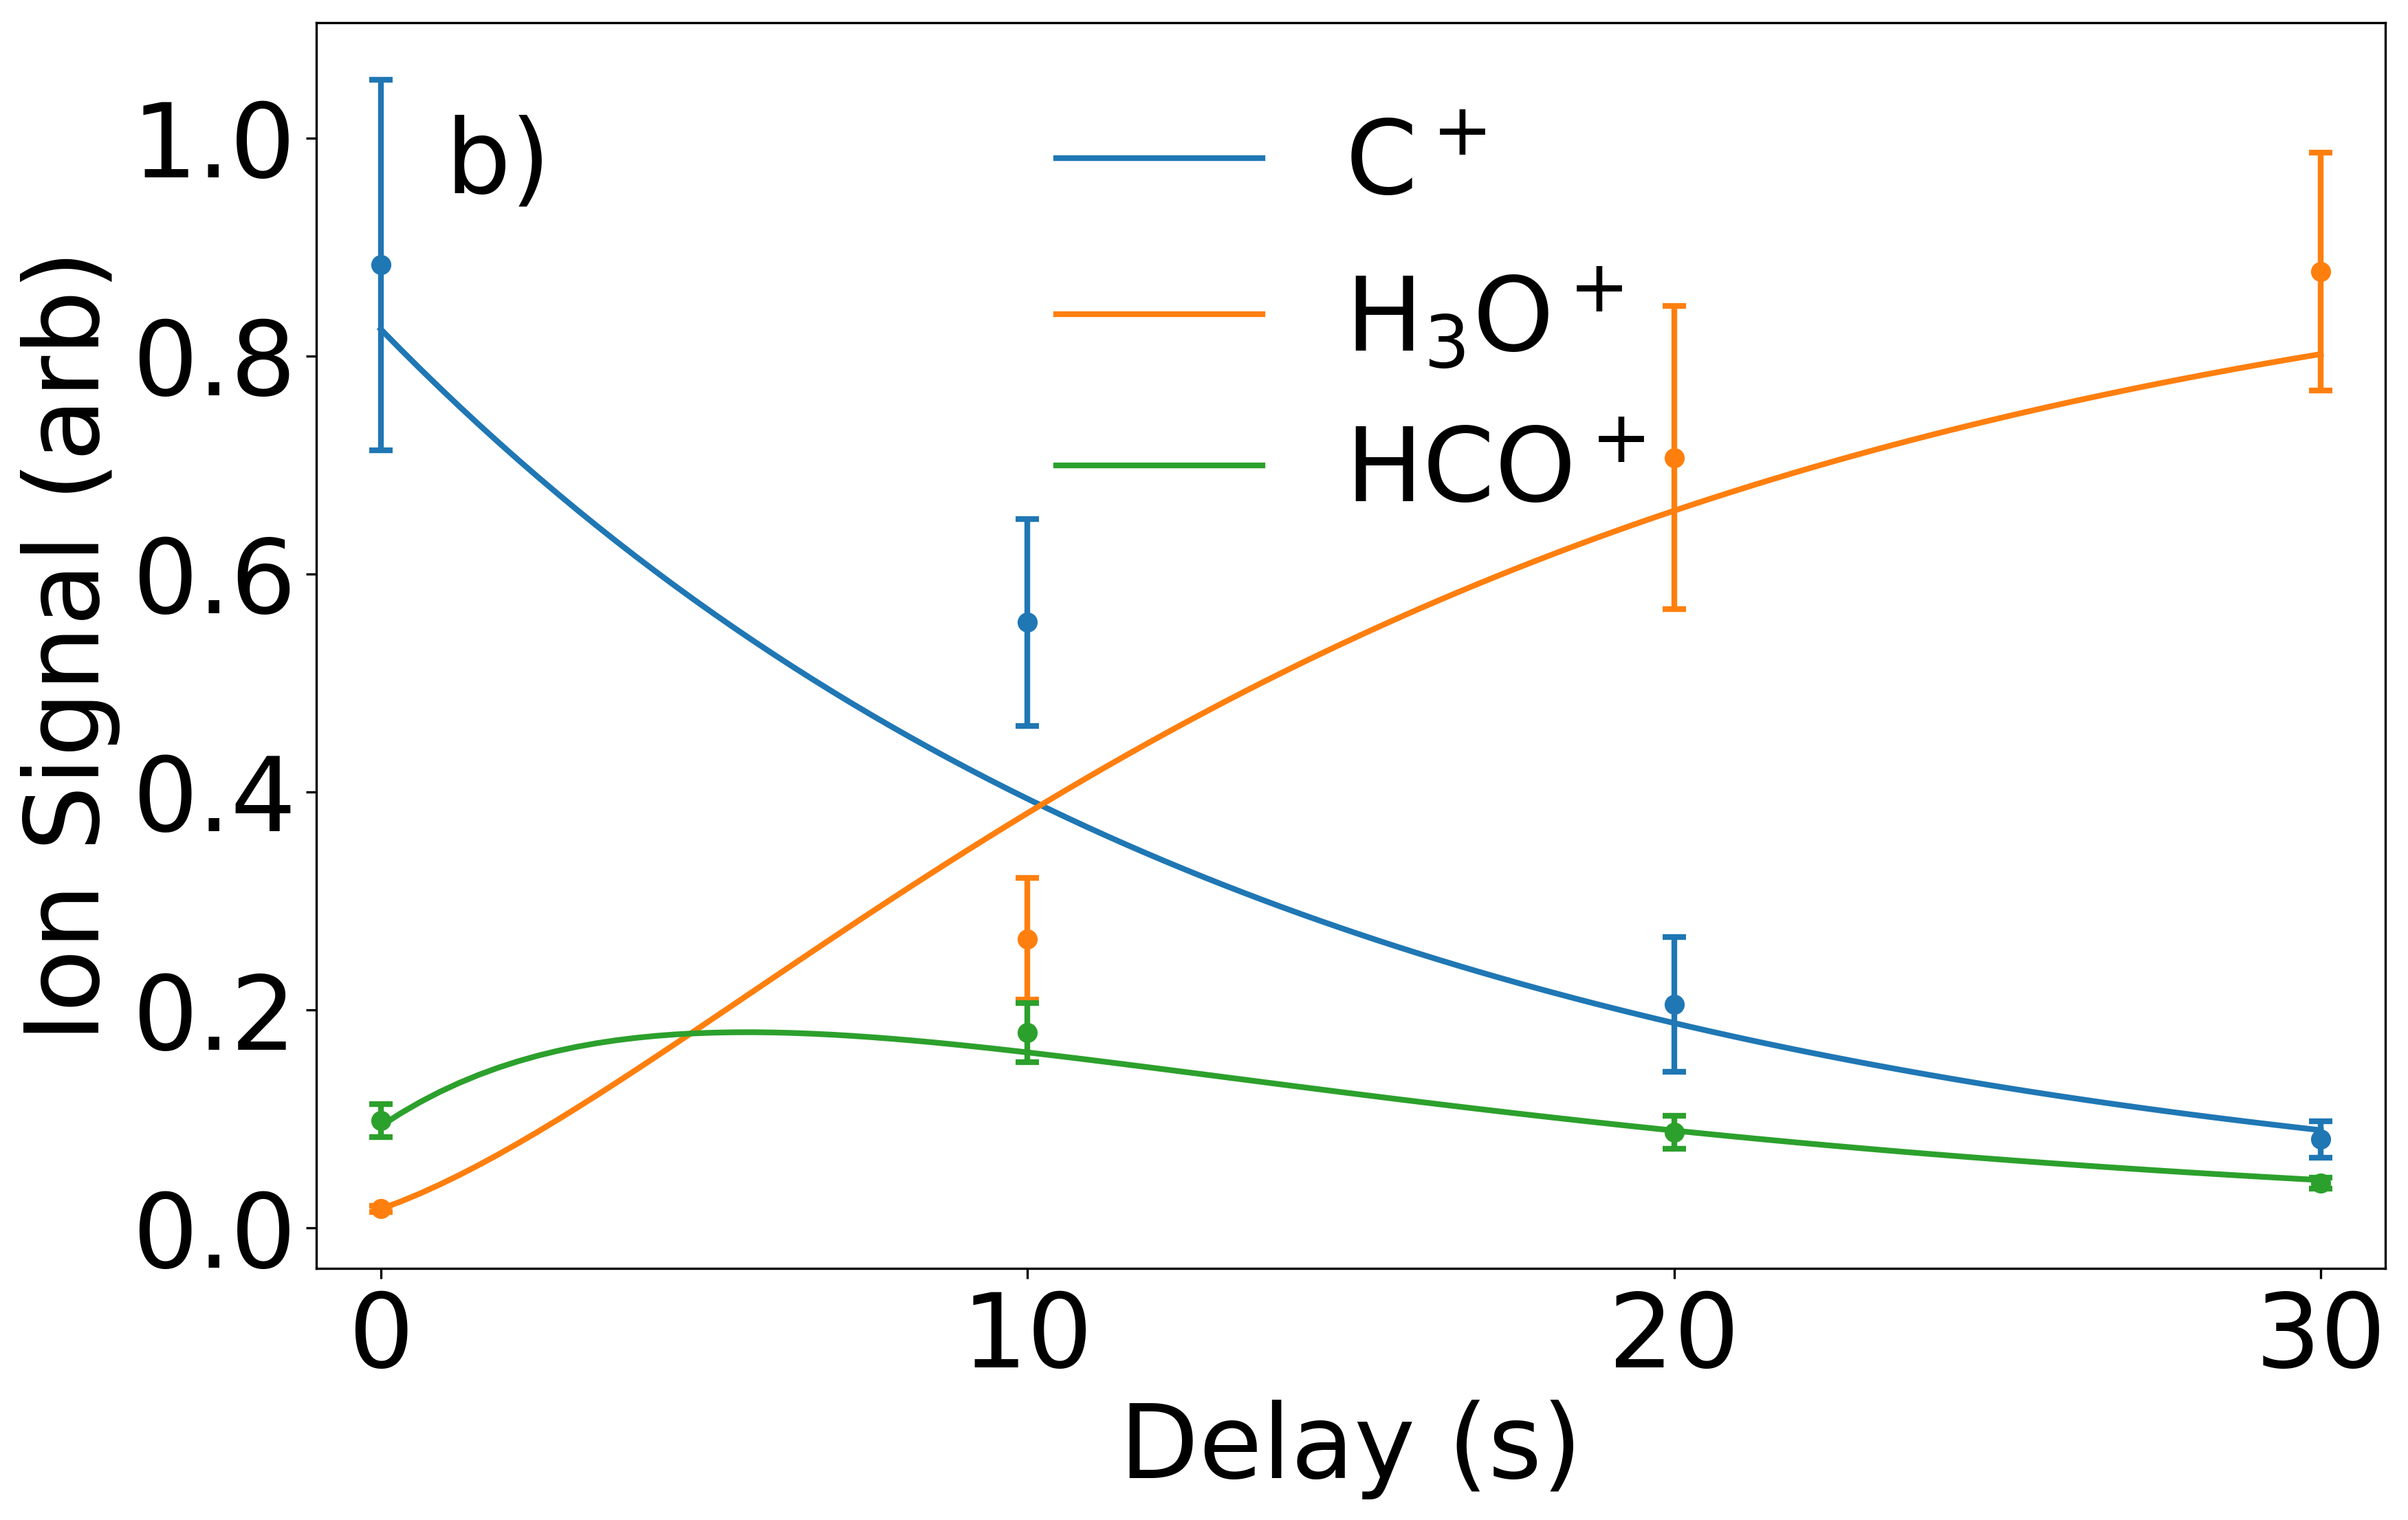
\includegraphics[width=0.5\textwidth]{images/C_H2O_CO_beam_traces_small.png}
	\end{tabular}
	}
	\caption{Time evolution of \ce{C+} and \ce{H2O} introduced via CBGB as well as subsequent reaction products. a) TOF traces without flooding of \ce{CO} where fitted rate constants are found to be $k_{\ref{r: C+H2O->HCO}}+k_{\ref{r: C+H2O->HOC}} = (7.7 \pm 0.6) \times 10^{-9}$ cm$^3$/s, and $k_{\ref{r: HCO+H2O->H3O}} = (1.7 \pm 0.2) \times 10^{-8}$ cm$^3$/s. b) TOF traces with flooding of \ce{CO} where fitted rate constants are found to be $k_{\ref{r: C+H2O->HCO}}+k_{\ref{r: C+H2O->HOC}} = (7.9 \pm 0.6) \times 10^{-9}$ cm$^3$/s, and $k_{\ref{r: [HCO]+H2O->H3O}} = (1.7 \pm 0.2) \times 10^{-8}$ cm$^3$/s.}
	\label{fig: [HCO]+H2O rate}
\end{figure}

Although we cannot make a statement about the rate of reaction \ref{r: HOC+H2O->H3O}, we see that at whatever ratio the isomers are produced, we cannot experimentally observe any meaningful deviation between the pure \ce{HCO+ + H2O} and \ce{[HCO]+ + H2O}. Thus, we find it reasonable to combine reactions \ref{r: HCO+H2O->H3O} and \ref{r: HOC+H2O->H3O} into:

\begin{equation}
\ce{[HCO]+ + H2O -> H3O+ + CO} \label{r: [HCO]+H2O->H3O}
\end{equation}

Where \ce{[HCO]+} is used to represent both isomers. With this understanding, we may take the ratio of isomers at $m/z=29$ to be constant with respect to time exposed to the beam.